\newpage
\chapter{Методы обучения с подкреплением в задаче управления} \label{ch2}
	
% не рекомендуется использовать отдельную section <<введение>> после лета 2020 года
%\section{Введение} \label{ch2:intro}

 
Обучение с подкреплением предлагает мощные алгоритмы разработки оптимального управления для систем с нелинейностями, со сложной неизвестной стохастической динамикой. Данная глава охватывает подходы RL с точки зрения инженера по управлению. В этой главе приводятся объяснения, как аппроксимация позволяет использовать RL с непрерывными состояниями и управляющими воздействиями.
Цель данной главы -- преодоление рассогласованности терминологии управления и RL.


\section{Переход между нотациями} \label{ch2:title-abbr} %название по-русски

Анализ динамических систем с использованием механики Лагранжа, Гамильтона, позволяет получить описание системы в форме нелинейных ОДУ или разностных уравнений. В первом случае объект управления описывается уравнением вида: 
\begin{equation*}
	\dot x = f(x, u),
\end{equation*}
где  $x(t) \in X \subseteq R^n$, $u(t) \in U \subseteq R^m$ -- управление.

Показатель качества (критерий оптимальности), по которому проектируется система управления, задается в виде:
\begin{equation*}
	J=\int_{0}^{t_f} L(t, x(t), u(t))dt + h(x(t_f), t_f),
\end{equation*}
где $t_f$ -- конечное время.

Такое представление системы, в отличии от МППР, имеет непрерывное пространство состояний, непрерывный вход, а так же непрерывность во времени. 

Во втором случае система либо дискретна по своей природе, либо приводится к дискретной форме: 
\begin{equation*}
x_{k+1} = f(x_k, u_k), \space  k=0, 1,.., N,
\end{equation*}

При этом выполняется свойство марковости, так как состояние в момент времени $k+1$ зависит только от состояния и входов в момент времени $k$. При этом $x_k$ и $u_k$ могут принадлежать конечному или счетному множеству, а так же континууму.
Показатель качества для дискретных систем имеет вид:
\begin{equation}
\label{eq:J_cost}
J = g_N(x_N) + \sum_{k=0}^{N-1} g_k(x_k, u_k),
\end{equation}
где \(g_N(x_N)\) -- терминальные (конечные) значения, N  -- число временных шагов (этапов, стадий)

В некоторых задачах важно получить представление об оптимальном процессе при длительном, практически неограниченном процессе. Отдельно выделяют задачи оптимального управления с бесконечным временем, когда $t_f\xrightarrow{}\infty$ или $N \xrightarrow{} \infty$. Особенность таких задач связана с тем, что показатель качества представляет собой бесконечную сумму или несобственный интеграл. 
Одни из наиболее распространенных подходов для задач с бесконечным временем является введение дисконтирования:
\begin{equation*}
	J = \int_{0}^{\infty} L(x(t), u(t))dt
\end{equation*}
или в дискретном случае:
\begin{equation*}
	J = \sum_{k=0}^{\infty} \gamma^{k}r(x_k,u_k)
\end{equation*}
где $0 < \gamma \leq 1$ - коэффициент дисконтирования.
Введение коэффициента дисконтирования гарантирует сходимость ряда или интеграла в большинстве случаев. Физический смысл — штраф или награда в будущем имеют меньшую значимость, чем текущая. Кроме того, введение дисконтирования уменьшает влияние неточности модели на показатель качества.

Рассмотрим переход от разностных уравнений к МППР и обратно. Пусть задан МППР:
\begin{equation*}
	p_{ij}(u,k)= P\{x_{k+1} = j |x_k = i, u_k = u\}
\end{equation*}
Соответствующая дискретная система будет $s_{k+1} = w_k$, где 
\begin{equation*}
{P\{w_k = j |x_k = i, u_k = u\} = p_{ij}(u_k)}
\end{equation*}
В обратную сторону, пусть задана дискретная система:
\begin{equation}
x_{k+1} = f(x_k, u_k, w_k)
\end{equation}
где $w_k \sim P_k(w_k|x_k,u_k)$ -- известно. Тогда
\begin{equation}
p_{ij}(u,k)= P_k\{W_k(i, u, j) |x_k = i, u_k = u\}
\end{equation}
где $W_k(i, u, j) = {w|j = f_k(i, u, w)}$

Как видно, в обучении с подкреплением обычно в общем случае рассматриваются стохастические системы, однако, для простоты, в данной работе ограничимся рассмотрением только детерминированных систем.

\section{Обучение с подкреплением для дискретных систем}

\textit{Классическое динамическое программирование}. Все задачи ДП направлены на работу динамических систем с дискретным временем. В детерминированных системах \(x_{k+1}\) определено. 
Задача ДП рассматривает динамические системы с дискретным временем вида:
\begin{equation}
x_{k+1} = f_k(x_k, u_k),
\end{equation}
где $k=0, 1,.., N-1$.

Цель -- найти управление, минимизирующее показатель качества:
\begin{equation}
\label{eq:J_cost}
J(x_0;u_0,...,u_{N-1}) = g_N(x_N) + \sum_{k=0}^{N-1} g_k(x_k, u_k),
\end{equation}
Тогда оптимальное значение функционала записывается как:
%
\begin{equation}
\label{eq:J_cost_min}
J^*(x_0) = \min_{\substack{u_k \in U_k(x_k) \\ k=0,...,N-1}} J(x_0;u_0,...,u_{N-1}),
\end{equation}

При решении задачи \eqref{eq:J_cost_min} методом ДП, поиск последовательности $J^*_N(x_N), J^*_{N-1}(x_{N-1}),..., J^*_0(x_0)$ осуществляется следующим образом:
\begin{equation*}
	J^*_N(x_N) = g_N(x_N) \text{ для всех }x_N
\end{equation*}
\begin{equation*}
	J^*_k(x_k) = \min_{u_k \in A_k(x_k)} [g_k(x_k, u_k) + J^*_{k+1}(f_k(x_k, u_k))] \text{ для всех } x_k
\end{equation*}

После этого, зная $J^*_{N}(x_{N}), J^*_{N-1}(x_{N-1})..., J^*(x)$, можно последовательно найти $u_0, ..., u_{N-1}$:


\begin{equation*}
	u^{*}_k \in \underset{u_k \in U_k(x^*_k)}{\arg \min}[g_0(a^*_k, x_k) + J^*_{k+1}(f_k(x^*_k, u_k))],
\end{equation*}
\begin{equation*}
	x^*_{k+1} = f_k(x^*_k, u^*_k),
\end{equation*}

Таким образом, для нахождения $u_0, ..., u_{N-1}$ необходимо вычисление всех $J^*_k(x_k)$. На практике вычисление \(J^*_k\) с помощью ДП занимает большое количество времени, поскольку количество \(x_k\) и \(k\) может быть очень большим. Главным недостатком метода является «проклятие размерности» –- сложность вычислений возрастает с увеличением размерности задачи. Помимо этого формирование управляющего воздействия методом ДП протекает не в режиме реального времени (режим off-line). С ростом сложности системы возникает необходимость хранения огромного количества данных, увеличение доли шумов. Решение задачи оптимального управления методом ДП, предполагает знание модели объекта, в следствии чего качество регулятора зависит напрямую от качества построения математической модели объекта. Отсутствие универсального алгоритма, который был бы пригоден для решения всех задач рассматриваемого класса. Алгоритмы ДП объединены общей идеей, но в каждом конкретном случае должны формироваться применительно к специфике прикладной задачи, поэтому отсутствие универсального алгоритма -- еще один недостаток методов оптимального управления, таких как ДП.


\section{Бесконечное время и методы}
Рассмотрим стационарную систему $x_{k+1} = f(x_k, u_k)$ на бесконечном интервале времени:
\begin{equation}
\label{f: fun_inf}
J = \sum_{k=0}^\infty g(x_k, u_k)
\end{equation}

Необходимо найти закон управления $\mu (x)$, который является также стационарным, что значительно упрощает синтез и реализацию. С другой стороны, в случае рассмотрения систем на бесконечном интервале времени мы не можем итеративно двигаться назад, начиная с терминального состояния, как мы это делали в случае конечного времени.
Обозначим как $J_{\mu} (x_0)$ значение функционала при законе управления $\mu$ и начальном условии $x_0$ . Тогда:
\begin{equation*}
	J_{\mu}(x_k) = \sum_{t=k}^{\infty} g(x_t, \mu(x_t)) = g(x_k,\mu(x_k)) + J_\mu(x_{k+1}), \space J_{\mu}(0) = 0
\end{equation*}
произведена замена бесконечного суммирования в \ref{f: fun_inf} на решение разностного уравнения. Отсюда можно получить следующий алгоритм решения рассматриваемой задачи, называемый итерации по ценности (VI):
\begin{equation*}
	\begin{matrix}
		J_0(x) = 0 \\
		J^*_{k+1}(x) = \underset{u_k \in U(x)}{\min}{[g_k(x_k, u_k) + J^*_{k}(f_k(x_k, u_k))]}, \space k = 0, 1, ...
	\end{matrix}
\end{equation*}

Рассмотренный выше алгоритм для конечного случая — тоже VI. Тот же самый алгоритм, переписанный в более привычном для RL виде:

Итерация по ценности:
\begin{enumerate}[1.]
	\item Инициализация. Выбор произвольного закона управления $\mu_0(x)$, $k=0$ и $J_0(s)$
	\item Шаг policy evaluation (оценка политики).
	\begin{equation*}
		J_{k+1}(x):=g(x, \mu_k(x)) + J_k(f(x,u))
	\end{equation*}
	
	\item Шаг policy improvement (обновление политики). Обновление закона управления
	\begin{equation*}
		\mu_{k+1}(x) =  \underset{\mu(\cdot)}{\arg\min}(g(x, \mu_k(x)) + J_{k+1}(f(x,u)))
	\end{equation*}
\end{enumerate}

Другой алгоритм -- итерация стратегии (PI):

\begin{enumerate}[1.]
	\item Инициализация. Выбор произвольного закона управления $\mu_0(x)$, $k=0$ и $J_0(s)$
	\item Шаг policy evaluation (оценка политики).
	\begin{equation*}
		J_{\mu_{k+1}}(x)=g(x, \mu_k(x)) + J(f(x,\mu_k(x)))
	\end{equation*}
	
	\item Шаг policy improvement (обновление политики). Обновление закона управления
	\begin{equation*}
		\mu_{k+1}(x) =  \underset{\mu(\cdot)}{\arg\min}(g(x, \mu_k(x)) + J(f(x,\mu_k(x))))
	\end{equation*}
\end{enumerate}
%\textbf{Про разницу между ними, про GPI, про всякие сходимости}




Рассмотрим вариант PI алгоритма, в котором шаг оценки стратегии производится неточно, в частности, алгоритм начинается с некоторого $J_0$ и генерирует последовательность пар функций стоимости и закона управления ${J_k, \mu_k}$ следующим образом: учитывая $J_k$, мы генерируем $\mu_k$ в соответствии с:
\begin{equation*}
	\mu_{k}(x) =  \underset{\mu(\cdot)}{\arg\min}(g(x, u) + J_{k}(f(x,u)))
\end{equation*}
и тогда получаем $J_{k+1}$ при $m_k \geq 1$
\begin{equation*}
		J_{\mu_{k+1}}(x_0)=J_k(x_{m_k}) + \sum^{m_k-1}_{t=0}g(x_t,\mu_k(x_t)))
\end{equation*}
где ${x_t}$ -- последовательность, сгенерированная с использованием $\mu_k$ и начиная с $x_0$, $m_k$ - произвольные положительные целые числа. При $m_k = 1$ алгоритм эквивалентен  алгоритму VI, а частный случай $m_k = \infty$ -- алгоритму PI. Такой алгоритм в RL называется Обобщенная итерация стратегий (Generalized Policy Iteration, GPI) -- одна итерация решения m-шагового уравнения Беллмана чередуется с шагом обновления политики). Алгоритм GPI при любом $m$ сходится к оптимальной стратегии и оптимальной оценочной функции.

\section{Приближенное динамическое программирование}
Эти методы широко распространены под названием приближенное или адаптивное динамическое программирование \cite{werbos1992approximate} или нейродинамическое программирование \cite{bertsekas1996neuro}.

Для преодоления  проклятия размерности применяют различные аппроксимации. Аппроксимировать можно $J_k^*$ (аппроксимация in value space) и или непосредственно управление (аппроксимация in policy space). Здесь важно привести еще одну важную классификацию в зависимости от то, когда вычисляется управление: оффлайн — вычисление управления производится до начала процесса управления, онлайн — вычисляем управление непосредственно в процессе эксплуатации. Так, аппроксимация in policy space — оффлайн метод, аппроксимация in value space — в основном онлайн метод.

В случае аппроксимации <<in policy space>> мы ищем управление из заданного параметрически семейства $\mu_k(x_k, r_k)$, где $r_k$ – параметры. Если осуществили аппроксимацию, то управление легко посчитать: $u_k = \widetilde{\mu}_k (x_k , r_k )$, то есть такой подход можно использовать для аппроксимации известного закона с целью удобного онлайн использования. В общем случае собираются пары $(x^s_k , u^s_k )$, $s = 1,..., q$, такие что u $s_k$ — хорошее управление для данного $x^s_k$ . Далее определяются параметры, например, методом наименьших квадратов.


В случае аппроксимации <<in value space>> аппроксимируем $J_k^*$  функцией
$\widetilde{J}_k$ . Тогда управление находится алгоритмом ДП, минимизируя функционал на конечном горизонте плюс аппроксимация оптимальной будущей стоимости $\widetilde{J}$. Значение $\widetilde{J}$  может быть получено разными способами: симуляция методами Монте-Карло, эвристики и др.

Методы нахождения $\widetilde{J}_k$ можно условно классифицировать на 4 группы:

\begin{enumerate}[1.]
	\item \textit{Аппроксимация задачи}. Нахождение функции $\widetilde{J}_k$ в более простой задаче. Вводится ряд допущений -- уменьшение размера пространста состояния, не учитываются нелинейности и т.д. Частный случай -- агрегация;
	\item \textit{Приближенная онлайн оптимизация}. Здесь применяются окононные алгоритмы: (Алгоритм Rollout algorithms, Model Predictive Control и т.д);
	\item \textit{Параметрическая аппроксимация}. Параметризуем $\widetilde{J}_k(x_k, r_k)$ некоторой параметрической функцией, где параметры определены используя данные и, например, нейронные сети;
	\item \textit{Агрегация}. Эта группа методов обычно предполагает разбиение пространства состояний. Более того, агрегация может применяться вместе с методами (1-3) и служить начальным приближением для решения задачи другим методом.
\end{enumerate}

В данной работе остановимся на 2 и 3 подходе.


\textit{Приближенная онлайн оптимизация, метод MPC}

Идея метод состоит в том, чтобы не параметризовать политику управления параметрами $W$ (как это будет далее показано в RL), а вместо этого оптимизировать входные данные управления $u_k$ непосредственно на конечном горизонте $T$. Чтобы учесть усеченный горизонт, мы можем использовать функцию ценности при некотором законе управлении, чтобы чтобы приблизить стоимость за пределами T шагов. Таким образом, политика управления определяется выражением
\begin{equation*}
	\mu_(x_k) = \underset{\mu(\cdot)}{\arg\min}(g(x_k, u)  + J(f(x,\mu_k(x))))
\end{equation*}

Модельное прогнозирующее управление (англ. model predictive control, MPC) -- метод управления который позволяет расчитывать управляющее воздействия на основе  математической модели объекта, прогнозируя значения переменных состояния и выхода, решая задачи оптимизации в реальном времени, при этом учитывая ограничения (\firef{fig:mpc-ch2}). Регулятор минимизирует ошибку между предсказанным и фактическим значением по горизонту управления. В отличии от классических подходов управления MPC позволяет управлять близко к ограничениям, что ведет к более устойчивой работе.

\begin{figure}[ht!] 
	\centering
	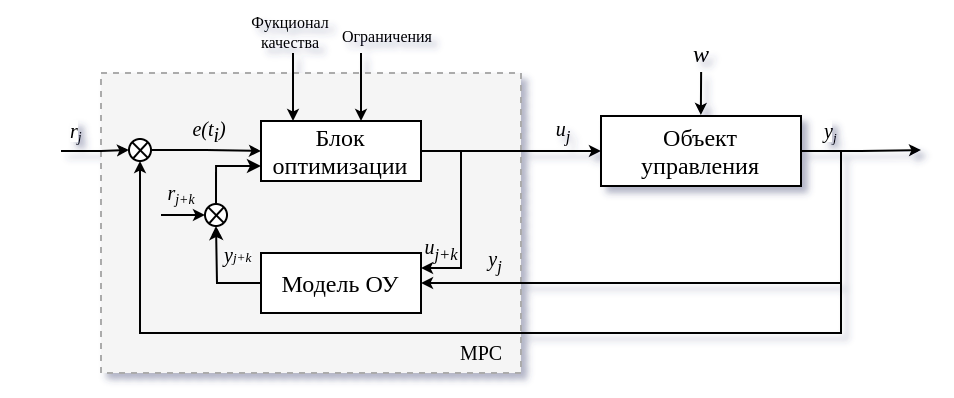
\includegraphics[width=0.9\linewidth]{my_folder/figure/schema/MPC.png}
	\caption{Структурная схема системы управления с прогнозирующими моделями}
	\label{fig:mpc-ch2}
\end{figure}


Регулятора на основе MPC получили широкое распространение в силу развития вычислительных мощностей. Отметим ключевые моменты, которые отличают подход MPC и RL: а) Так как на каждом шаге решается задача оптимизации, качества управления во многом будет зависеть от точности модель процесса. В то время как регуляторы RL не требуют какого-либо предварительного доступа к модели процесса: б) Промышленные системы управления подвержены эксплуатационным ограничениям, которые должны всегда соблюдаться. MPC устраняет эти ограничения, явно включая их в задачу оптимизации, решаемую на каждом этапе. В контроллере RL ограничения могут быть встроены непосредственно в функцию перенастройки или реализованы посредством отсечения градиента. Второй подход более мягкий -- нарушение ограничения может произойти во время обучения, но оно не приветствуется из-за огромного штрафа в сигнале вознаграждения. Надежные механизмы для безопасной работы полностью обученной системы и, действительно, для безопасной работы во время онлайн-обучения, являются открытой задачей для RL регулирования.
в) Адаптация: со временем меняются параметры систем. Поддержание производительности требует реагирования как на изменения, так и на неизвестные нарушения. Традиционные системы на основе MPC включают механизмы для
выявление несоответствия модели и объекта, но изменение параметров будет сопровождаться повторной идентификацией модели процесса. Этот процесс, который требует одновременной оценки состояния и параметров, может быть сложным и дорогостоящим. Некоторые недавние варианты MPC, такие как робастный MPC и стохастический MPC, учитывают неопределенности модели, встраивая их непосредственно в задача оптимизации. Регуляторы на основе RL автоматически корректируют параметры в сетях актеров и исполнителях. Это обеспечивает регулятор RL свойством самонастройки, так что процесс остается субоптимальным по отношению к выбранному критерию вознаграждения.



Рассмотрим \textit{параметрическую аппроксимацию}. Для этого представим оценку функции стоимости в следующем виде:
\begin{equation*}
	\label{f:approx_val_funt}
	\widetilde{J}_\mu(x) = W^T\varphi(x)
\end{equation*}
где базисный вектор $\varphi(x) = [\varphi_1(x), \varphi_2(x), ... \varphi_L(x)]$, $W \in \mathrm{R}^L$ --вектор настраиваемых параметров. Для наивной настройки весов W
требуется для каждого $x_k$ вычислять $\widetilde{J}_\mu(k)$, то есть вычисления производятся оффлайн. Для устранения этого недостатка вводится понятие временного различия (англ, Temporal Differences, TD):
\begin{equation*}
	e_k = g(x_k,\mu(x_k)) + J_{\mu}(x_{k+1}) - J_{\mu}(x_k)
\end{equation*}

Если $e_k = 0$ для всех $x_k$ , то это просто уравнение Беллмана. TD ошибка представляет собой ошибку между предсказанной и действительной наградой за действие. Это равенство должно выполняться для всех $x_k$ в любой
момент времени $k$, поэтому можно записать онлайн версии рассмотренных ранее алгоритмов.

\textit{Онлайн алгоритм итерации по стратегии (онлайн PI)}

\begin{enumerate} [1.]
	\item \textit{Инициализация}. Выбор любого допустимого закона управления $\mu_0(x_k)$
	\item \textit{Шаг оценки стратегии}. Оценка параметров $W_{j+1}$:
	\begin{equation*}
		\label{f:policy_iteration_online}
		W^T_{j+1}(\varphi(x_k) - \gamma \varphi(x_{k+1})) = r(x_k, h_j(x_k))
	\end{equation*}
	\item  \textit{Шаг улучшения стратегии}. Обновление закона управления:
	\begin{equation*}
		\mu_{j+1}(x_k) = \underset{\mu(\cdot)}{\arg\min}(g(x_k, \mu(x_k)) + W^T_{j+1}\varphi(x_{k+1}))
	\end{equation*}
\end{enumerate}


\textit{Онлайн алгоритм итерации по ценности. (онлайн VI)}
\begin{enumerate} [1.]
	\item \textit{Инициализация}. Выбор любого закона управления $\mu_0(x_k)$, не обязательно допустимой.
	\item  \textit{Шаг оценки стратегии}. Оценка параметров $W_{j+1}$:
	\begin{equation}
	\label{f:value_iteration_online}
	W^T_{j+1}\varphi(x_k) =g(x_k, \mu_j(x_k)) + W^T_{j}\gamma \varphi(x_{k+1})
	\end{equation}
	\item  \textit{Шаг улучшения стратегии}. Обновление закона управления:
	\begin{equation*}
		\mu_{j+1}(x_k) = \underset{\mu(\cdot)}{\arg\min}(g(x_k, \mu(x_k)) + W^T_{j+1}\varphi(x_{k+1}))
	\end{equation*}
\end{enumerate}

В обоих алгоритмах на шаге policy evaluation, параметры $W_{j + 1}$ можно искать методом наименьших квадратов. Однако для этого требуется обновление закона управления производить не раньше, чем через $L$ шагов с этим законом. Так как $W_{j + 1} \in R^L$ , нужно не менее $L$ уравнений для оценки этого вектора. В момент времени $x_{k+1}$ имеем набор $(x_k , \mu_(x_k), x_{k+1} , g(x_k , \mu(x_K)))$, то есть одно уравнение. Однако обычно вектор параметров $W_{j + 1}$ ищут рекурсивным методом наименьших квадратов или градиентным спуском до сходимости, а затем обновляют закон управления.

На шаге обновления закона управления необходимо осуществлять поиск функции, что плохо, поэтому необходимо параметризовать. Параметризовав шаг 3,получаем схему исполнитель-критик.

Часто реализация обучения с подкреплением осуществляется с использованием двух НС: одна в качестве критика, а другая в качестве исполнителя (рисунок 1). В этой системе управления критик и исполнитель настраиваются в режиме онлайн с использованием наблюдаемых данных. Критик и исполнитель настраиваются последовательно -- веса одной НС остаются постоянными, а веса другой настраиваются до сходимости. Эта процедура повторяется до тех пор, пока обе НС не сойдутся. Затем регулятор определяет оптимальное значение управления в режиме онлайн. Таким образом,
это онлайн оптимально-адаптивная система управления, в которой параметры аппроксимированного функционала настраиваются онлайн, обеспечивая сходимость к оптимальному управлению.
%
\begin{figure}[ht!] 
	\centering
	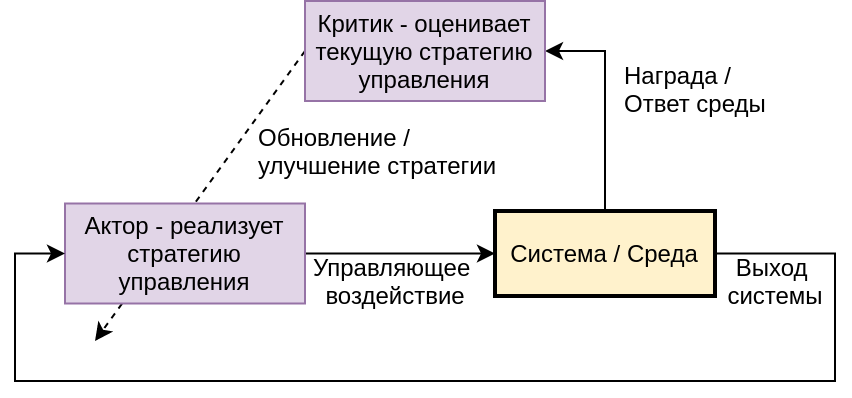
\includegraphics[width=0.8\linewidth]{my_folder/figure/schema/actor_critic.png}
	\caption{Структурная схема системы управления с прогнозирующими моделями}
	\label{fig:my_label}
\end{figure}
%
%
\section{Q-фактор}
На данном этапе получили онлайн версии с параметризацией, но в описанных выше алгоритмах, даже если мы знаем $J$, требуется знать функцию $x_{k+1} = (x_k, u_k)$. То есть все еще требуется построение модели. Поэтому вводим понятие Q-фактора.

Можно ввести следующее обозначение:
\begin{equation*}
	Q^*_k(x_k, u_k)= g_k(x_k, u_k) + J^*_{k+1}(f_k(x_k, u_k))
\end{equation*}
Тогда
\begin{equation*}
	u_k^* \in \underset{u_k \in U_k(x_k^*)}{\arg \min}Q^*_k(x_k^*, u_k)
\end{equation*}

Оптимальная стоимость записфвается как:
\begin{equation*}
	J_k^*(x_k) = \underset{u_k \in U_k(x_k^*}{\min}Q^*_k(x_k, u_k)
\end{equation*}

Тогда алгоритм ДП можно переписать через Q-фактор:
\begin{equation*}
	Q_k^*(x_k, u_k) = g_k(x_k, u_k) + \underset{u_{k+1} \in U_{k+1}(f_k(x_k, u_k))}{\min}Q^*_{k+1}(f_k(x_k, u_k), u_{k+1})
\end{equation*}

$J$ имеет преимущество, что если система меняется, то работает (online replanning).





Оптимальные методы управления обычно направлены на поиск закона управления в автономном режиме при условии наличия базовых динамических моделей. Когда лежащие в основе модели недоступны или известны только частично, используются подходы адаптивного управления в онлайн режиме \cite{landau2011adaptive}. Таким образом, можно сказать, что онлайн-методы RL -- это методы адаптивного оптимального управления. Так как RL направлено на поиск оптимального (субоптимального) закона управления в режиме онлайн с использованием измерений в реальном времени без знания модели системы.

Анализ устойчивости оптимальных и адаптивных методов управления имеет решающее значение в потенциально опасных приложениях, например, при взаимодействии человека и робота, автономная робототехника или управление электростанциями. При разработке оптимальных и адаптивных законов управления на первом этапе выбираются детерминированные настройки.
Впоследствии, потенциальные неопределенности (шумы и возмущения) которые не учтены в детерминированной настройке, исследуются с использованием различных инструментов устойчивости, чтобы сделать вывод об устойчивости, например, о локальной, асимптотической, экспоненциальной устойчивости.

В отличие от стандартных подходов в управлении, которые с самого начала ставят требования полной устойчивости, подходы RL требуют дополнительных гарантий стабильности и надежности. Стоит отметить, что здесь нас интересует устойчивость с точки зрения управления, то есть устойчивость замкнутой системы в результате управления. Тогда как в ИИ, термин устойчивость относится к сходимости алгоритмов обучения (к асимптотическому поведению с точки зрения управления). 
Это подчеркивает философское различие между искусственным интеллектом и областью автоматического управления. Исследователи ИИ сосредотачиваются на производительности с точки зрения совокупного вознаграждения, где вознаграждение может иметь любое значение и рассматривается как часть задачи. Алгоритмически это означает, что учитывается только сходимость (качественная / асимптотическая или количественная через скорости сходимости) процесса обучения к почти оптимальному решению, в то время как допустимые границы в процессе обучения, которые необходимы для обеспечения устойчивости замкнутого контура, не учитываются. Иногда это допустимо в силу характера некоторых приложений ИИ (например, для обработки видео или настольных игр). Цели инженеров по управлению направлены на соблюдение устойчивости, так что даже при использовании оптимального управление главная - и часто единственная - роль фунции стоимости заключается в уточнениях требований устойчивости, например, в стандартных подходах к MPC.

%С этой точки зрения шаг улучшения политики в Разделе 2.3.1.2
%можно рассматривать как явную схему прогнозирующего управления моделью, %которая приближает модель прогнозирующей политики управления $\mu(x)$ в %(2.11) с параметрической политикой πθ


\section{Обучение с подкреплением для непрерывных систем}

Для систем с непрерывным временем применение методов обучения с подкреплением  сложнее, чем для систем с дискретным временем. 

Рассмотрим нелинейную динамическую систему с непрерывным временем:
\begin{equation*}
	\dot x = f(x) + g(x)u
\end{equation*}
с состоянием $x(t) \in R^n$, управляющим входом $u(t) \in R^m$,  Предполагается, что система стабилизируема на $\Omega$ -- существует непрерывное управляющее воздействие $u(t)$ такое, что замкнутая система асимптотически устойчива на $\Omega$.


Задана мера производительности или функции стоимости, связанной с политикой управления обратной связью $u = \mu(x)$ как:
\begin{equation*}
	J^{\mu}(x(t)) = \int_t^\infty{r(x(\tau),u(\tau))d\tau}
\end{equation*}
где награда $r(x,u) = Q(x) + u^TRu$ и $Q(x)$ -- положительно определенная.
Уравнение Беллмана определяется на основе Гамильтонина:
\begin{equation*}
\label{f:hamiltonianC}
H(x, \mu(x), \nabla J^{\mu}) = r(x, \mu(x)) + (\nabla J^{\mu})^T (f(x)+g(x) \mu(x)))
\end{equation*}
где $\nabla J^{\mu}$ -  градиент функции стоимости $J_m$ по отношению к $x$
Отметим проблемы с непрерывными системами: сравним Гамильтониан для непрерывных систем Беллмана с Гамильтонианом для дискретных систем. Первый содержит полную динамику системы $f(x) + g(x)u$, а Гамильтониан для дискретных систем - нет. Это означает, что нет возможности использовать уравнение Беллмана в качестве основы для обучения с подкреплением, если не известна полная динамика.

Было проведено несколько исследований обучения с подкреплением, где применялся метод Эйлера для дискретизации уравнения Беллмана
\begin{equation*}
0 = r(x,\mu(x)) + (\nabla V^{\mu})^T(f(x) + g(x)\mu(x)) = r(x, \mu(x))+V^{\mu}
\end{equation*}
%
\begin{gather*}
	0 = r(x_k, u_k) + \frac{V^\mu(x_{k+1} - V^{\mu}(x_k)}{T} =\\
	= \frac{r_S(x_k, u_k}{T} + \frac{V^{\mu}(x_{k+1} - V^{\mu}(x_k)}{T}
\end{gather*}
с периодом $T$ так, чтобы $t = kT$. Награда для дискретной формы $r_S(x_k, u_k) = r(x_k, u_k)T$ задается  через умножение на период $T$.


Дискретизированное уравнение  Беллмана имеет тот же вид, что и дискретное уравнение Беллмана . Следовательно, могут применяться все вышеописанные методы обучения с подкреплением.
\textit{Алгоритм итерации по стратегии для непрерывных систем}
\begin{itemize}
	\item \textit{Инициализация}. Выбор любой допустимой политики $\mu ^(0)(x)$.
	\item \textit{Шаг оценки стратегии}. Решение $V^{\mu^(i)}(x(t))$:
	\begin{equation}
	V^{\mu^(i)}(x(t)) = \int_t^{t+T} r(x(s), \mu^(i)(x(s))ds + V^{\mu^(i)}(x(t+T))
	\end{equation}
	где $V^{\mu^(i)}(0) = 0$
	\item \textit{Шаг улучшение стратегии}. Определение улучшенной стратегии:
	\begin{equation*}
		\mu^{i+1} = \underset{u}{\arg\min}[H(x, u, \nabla V^{\mu^{(i)}}_x)]
	\end{equation*}
\end{itemize}

\textit{Алгоритм итерации по ценности для непрерывных систем}
\begin{itemize}
	\item \textit{Инициализация}.Выбор любой политики управления $\mu ^(0)(x)$, необязательно допустимой.
	\item \textit{Шаг оценки стратегии}.
	\begin{equation}
	V^{\mu^(i)}(x(t)) = \int_t^{t+T} r(x(s), \mu^(i)(x(s))ds + V^{\mu^(i+1)}(x(t+T))
	\end{equation}
	\item \textit{Шаг улучшение стратегии}.
	\begin{equation*}
		\mu^{i+1} = \underset{u}{\arg\min}[H(x, u, \nabla V^{\mu^{(i)}}_x)]
	\end{equation*}
\end{itemize}

Стоит обратить внимание, что ни один алгоритм не требует знания динамики системы. То есть они работают для частично неизвестных систем.

\section{Обучение с подкреплением и адаптивное управление}

В настоящее время наблюдаются существенные отличия в терминологии области теории автоматического управления и обучения с подкреплением. Так в одном случае используется терминология, связанная с искусственным интеллектом - максимизация функции, ценность, награда, тогда как в случае ДП стандартным является терминология из области ТАУ - минимизация функции, стоимость, затраты (\taref{tab:RL_TAC}).
\begin{table}[h!]
	\centering
	\small
	\caption{Термины RL и ТАУ}
	\begin{tabular}{|l|p{250pt}|}
		\hline
		Обучение с подкреплением & Теория управления \\
		\hline
		Агент &  Алгоритм принятия решения, регулятор \\
		\hline
		Действие & Управляющее воздействие \\
		\hline 
		Среда & Объект управления (система) \\
		\hline
		Награда & Противоположна стоимости \\
		\hline
		Функция ценности & Противоположна функции стоимости (функционал качества) \\
		\hline
		Максимизация функции ценности & Минимизация функции стоимости \\
		\hline
		
	\end{tabular}
	\label{tab:RL_TAC}
\end{table}

На \firef{fig:NA-ch2} показано две структурные схемы, первая из которых свойствена в рамках теории управления, а вторая -- науке ИИ. Стоит отметить, что в терминологии ИИ в физический мир (окружение) относят все элементы и сигналы, не относящиеся к алгоритму регулятора -- объект управления, исполнительный механизм, датчики, задающие устройства, шум и т.д.
%
\begin{figure}[ht!] 
	\centering
	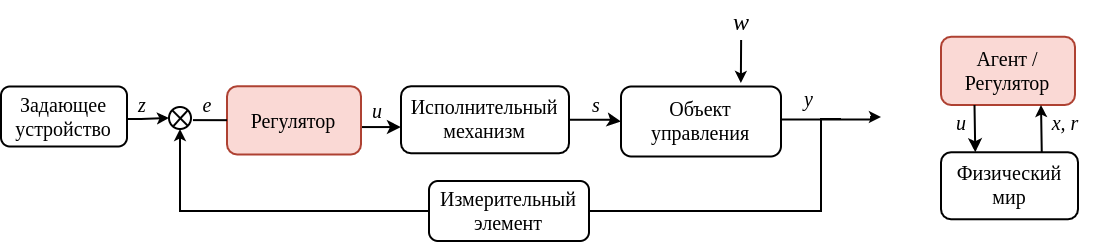
\includegraphics[width=0.8\linewidth]{my_folder/figure/schema/TAY_RL.png}
	\caption{Структурная схема системы управления}
	\label{fig:NA-ch2}
\end{figure}

\textit{Связь адаптивного управления и RL}

Косвенное адаптивное управление, включает блок идентификации, который принимает на вход управляющее воздействие и действительный выход с объекта управления, расчитывает новые параметры, чтобы обновить параметры управления.Данный подход похож на методы RL на основе модели. (\firef{fig:r_adap1-ch2})
%
\begin{figure}[ht!] 
	\centering
	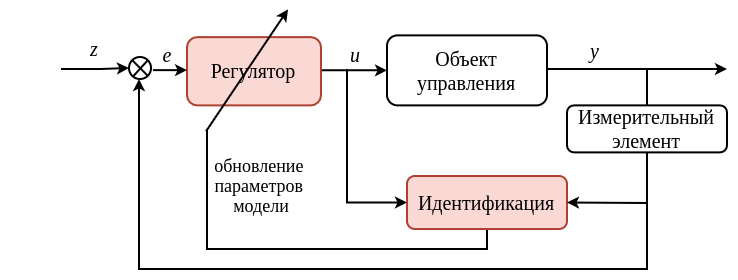
\includegraphics[width=0.8\linewidth]{my_folder/figure/schema/adapt1.png}
	\caption{Косвенное адаптивное управление или модельный RL}
	\label{fig:r_adap1-ch2}
\end{figure}
%

В этом случае идентификация представлена предсказывающим блоком и блоком оценки (\firef{fig:r_adap2-ch2}). На вход блока оценки поступает предсказанный сигнал и действительный сигнал, в случае, если различие между сигналами превосходит некоторого заданного порога, критик инициирует обновление параметров блока предсказателя. Данный подход аналогичен имитационному обучению, где цель RL формируется не на основе функции награды, а на основе экспертных около-оптимальных данных.
\begin{figure}[ht!] 
	\centering
	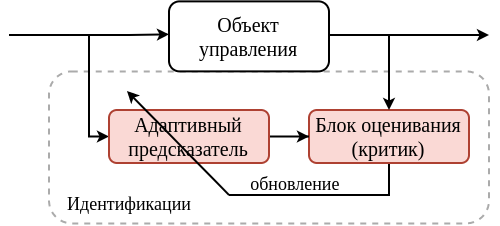
\includegraphics[width=0.4\linewidth]{my_folder/figure/schema/adapt2.png}
	\caption{Идентификация или имитационное обучение}
	\label{fig:r_adap2-ch2}
\end{figure}
%
В прямом адаптивном управлении явно не задается модель системы (\firef{fig:r_adap-ch2}), а используется специальный механизм для сравнения желаемого значения сигнала на выходе и действительно, при этом
Прямое адаптивное управление соответсвует безмодельному RL.
%
\begin{figure}[ht!] 
	\centering
	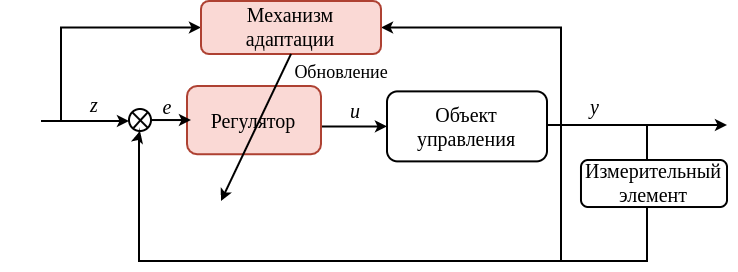
\includegraphics[width=0.4\linewidth]{my_folder/figure/schema/adapt3.png}
	\caption{Прямое адаптивное управление}
	\label{fig:r_adap-ch2}
\end{figure}
Рассмотрим один из основополагающих алгоритмов в RL -- итеративное обучение (\firef{fig:r_adap4-ch2}). Представим этот метод, используя две одинаковые замкнутые системы. Моделирование выполняется на разных итерациях. Первая система запускается на перой итерации, накапливая последовательность рассогласования, генерирует сигнал ошибки, подает его на вход регулятора, который генерирует поправку, на основе минимизации наблюдаемой ошибки. Поправка суммируется с управляющим сигналом регулятора второй система на другом шаге итерации. Такой процесс может выполнятся на каждой итерации с целью подавления помех в замкнутом контуре и минимизации ошибки управления.

\begin{figure}[ht!] 
	\centering
	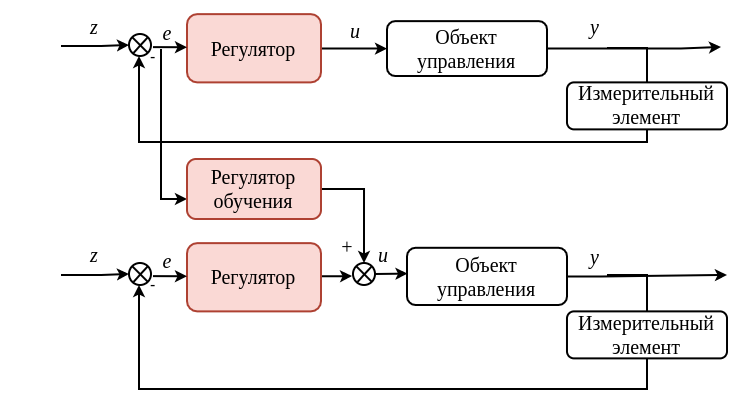
\includegraphics[width=0.6\linewidth]{my_folder/figure/schema/adapt4.png}
	\caption{Итеративное обучение}
	\label{fig:r_adap4-ch2}
\end{figure}


\section{Открытые задачи обучения с подкреплением}

Обучение с подкреплением доказало свою ценность в ряде ограниченных задач, но большую часть исследований в области RL часто трудно использовать в реальных системах из-за ряда допущений, которые редко выполняются на практике \cite{dulac2019challenges}. Ниже перечислены основные нерешенные задачи в области RL, которые необходимо решить, чтобы активно использовать методы RL для управления технических систем:
\begin{itemize}
\item Настройка регулятора на реальной системе на ограниченных образцах.
\item Многомерные непрерывные пространства состояний и действий.
\item Ограничения безопасности, которые никогда или, для определенных объектов, редко должны нарушаться.
\item Частично наблюдаемые системы, альтернативно рассматриваются как нестационарные или стохастические.
\item Сложность формализации функционала качества (функции награды), в частности, для многоагентных систем.
\item Интерпретируемость результатов синтеза регуляторов на базе RL.
\item Расчет управляющее воздействие на частоте работы системы.
\item Большие или неизвестные задержки в исполнительных или измерительных механизмах системы.
\end{itemize}
В отличие от большинства исследований в области RL, в реальных системах нет отдельной среды настройки и оценки. Все данные для обучения поступают из реальной системы, регулятор должен работать достаточно хорошо и действовать безопасно на протяжении всей настройки (обучения). Для многих систем это означает, что исследование должно быть ограничено, в результате поступающие данные будут иметь низкую дисперсию -- небольшая часть пространства состояний может быть исследована. Кроме того, поскольку часто существует только один экземпляр системы, подходы, которые создают экземпляры сотен или тысяч сред для сбора большего количества данных для распределенного обучения, не могут быть применены. В случае, если существуют собранные автономные данные по системе, в большинстве случаев они не содержат необходимое количество и охват, которые необходимы существующим алгоритмам RL. Итерации обучения в реальной системе могут занять много времени, так как есть некоторые системы с большим периодом управления -- от одного часа до нескольких месяцев, а ответный сигнал может составлять порядка месяцев (например, управление гидро- и литосферными процессами, онлайн-реклама, эффективность применения лекарственных препаратов). Даже в случае высокочастотных задач управления алгоритм обучения должен быстро настраиваться на потенциальных ошибках без необходимости повторять их несколько раз, прежде чем исправлять их. Таким образом, для обучения в реальной системе требуется, чтобы алгоритм был эффективным и производительным.

В области обучении с подкреплением выделают отдельное направление связанное с разработкой безопасных алгоритмов RL. Безопасное обучение с подкреплением можно определить как процесс разработки закона управления при максимизации функционала, при обеспечении соблюдение ограничений безопасности во время процессов настройки и эксплуатации. Как правило, выделяют два подхода к безопасному обучению с подкреплением.
Первый основан на модификации критерия оптимальности. Второй основан на модификации процесса обучения путем включения внешних знаний, дополнительных ограничений. Может применяется резервный регулятор, который в случае, если закон управления нарушает ограничения безопасности, взять на себя управление. Это своего рода алгоритмическое резервирование управления (\firef{fig:r_safe_rl-ch2})
\begin{figure}[ht!] 
	\centering
	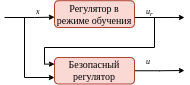
\includegraphics[width=0.4\linewidth]{my_folder/figure/schema/safe_RL.png}
	\caption{один из вариантов}
	\label{fig:r_safe_rl-ch2}
\end{figure}

Есть ряд успешных работ, которые изучают варианты использования функции Ляпунова для доказательства безопасности управления \cite{chow2018lyapunovbased}.

Еще одним важным аспектом реальных систем является то, что они принадлежат и управляются людьми, которые требуют понимания алгоритмов управления. По этой причине интерпретируемость закона управления важна для реальных задач. Особенно в случаях, когда функция имеет альтернативный и неожиданный подход к управлению. В случае ошибок алгоритма управления важно иметь возможность апостериорно понять причину ошибки. Есть ряд работ направленных на исследование данной проблемы, например, с применением предметно-ориентированного языка программирования.

Вывод по главе \thechapter. В ходе анализа и изучения связи между обучением с подкреплением и управлением, сделаны следующие выводы:
\begin{itemize}
	
	\item Обучение с подкреплением -- это параметрический метод аппроксимации функции ценности для решения задачи приближенного динамического программирования;
	\item Обучение с подкреплением, как и приближенное динамическое программирование способно справиться с проблемой проклятья размерности;
	\item Динамическое программирование рассматривается как один из главных способов обучения агента;
	\item Модельное обучение с подкреплением соответствует косвенному адаптивному управлению, безмодельное обучение с подкреплением соответствует прямому адаптивному управлению;
	\item Главные нерешенные задачи обучения с подкреплением -- это описание функции награды и обеспечение безопасности как во время настройки регулятора, так и во время эксплуатации;
\end{itemize}